%========================================================================
% Modelo para elaboracao de textos academicos: TCC, dissertacoes e teses
% Elaborado pelo GISIS - Grupo de Imageamento Sismico e Inversão Sismica.
%========================================================================
\chapter{Revisão Bibliográfica}
\label{ch:revisaobibliografica}

A modelagem e tomografia sísmica são técnicas essenciais na exploração de recursos naturais subterrâneos e na caracterização da subsuperfície terrestre. A tomografia sísmica é um método não invasivo que permite mapear as propriedades físicas do subsolo através da análise das ondas sísmicas geradas por fontes controladas. Um dos principais desafios na tomografia sísmica é a obtenção de informações precisas sobre as trajetórias das ondas sísmicas e suas velocidades de propagação em diferentes camadas geológicas. Nesse sentido, a equação \textit{eikonal}  é uma ferramenta fundamental para a modelagem e inversão e imageamento sísmico, pois descreve as frentes de onda e permite calcular os tempos de percurso das ondas sísmicas. Neste capítulo é explorado a equação eikonal, três resoluções numéricas e sua aplicação na tomografia de refração. Ao explorar esses tópicos, este capítulo fornecerá abrangentes conceitos utilizados na geração dos resultados deste trabalho.

\section{Modelagem sísmica}

Muitos fenômenos físicos tem suas simplificações e condições para serem simulados computacionalmente. O método sísmico parte do princípio da propagação de ondas mecânicas geradas a partir de uma fonte explosiva, sendo registradas em receptores posicionados na superfície da terra ou no fundo marinho \cite{sheriff1995exploration, rosa2010analise}. Um modelo de propriedades físicas de subsuperfície é necessário para a simulação computacional. Considerando a simplificação da equação da onda para meios acústicos e isotrópicos, onde a propriedade do meio são as velocidades da onda P, as frentes de onda podem ser geradas para realizar estudos sintéticos experimentais. Existem formatos de solução para uma equação que rege um fenômeno físico, dois deles são o caso analítica e o caso numérico. A solução analítica de um problema mostra a resposta exata do fenômeno em condições específicas previamente estabelecidas e a solução numérica resolve o problema de forma geral para diversos cenários. No caso da modelagem sísmica, as condições estabelecidas se aplicam ao modelo de velocidade, resolvendo a equação em um modelo homogêneo ou com camadas plano paralelas sem variação lateral de velocidade.  

\subsection*{Equação da onda para meios acústicos}

A equação base para a simulação sísmica utilizando a simplificação para meios acústicos pode ser formulada da seguinte maneira
\begin{equation}
	\nabla^2u(\mathbf{x}, t) - \dfrac{1}{v^2(\mathbf{x})}\dfrac{\partial^2u(\mathbf{x}, t)}{\partial t^2} = f(t),	
	\label{wave_equation}
\end{equation}
\noindent onde $u(\mathbf{x},t)$ é o campo de pressão hidrostática, $t$ é o tempo de propagação e $\mathbf{x} = (x,y,z)$ são as variáveis do sistema de coordenadas para o caso 3D. $v(\mathbf{x})$ é o modelo de velocidade, $f(t)$ é uma função que determina o formato do pulso propagado e $\nabla^2 = \partial_x + \partial_y + \partial_z$ é o operador laplaciano. \citeonline{igel2017computational} mostra algumas formas de resolver a equação da onda numericamente de forma prática e aplicada. O método das diferenças finitas é um dos métodos mais utilizados em simulações sísmicas. O princípio do método é estimar o valor da derivada numericamente utilizando a série de Taylor, definida detalhadamente no trabalho de \citeonline{de2005funccoes}. Somente derivadas de segunda ordem são necessárias para resolver a equação \ref{wave_equation} e a aproximação da derivada pode ser definida a partir da seguinte expressão
\begin{equation}
	\dfrac{\partial^2 f(x)}{\partial x^2} \approx \dfrac{f[i - dh] - 2f[i] + f[i + dh]}{dh^2},
	\label{derivada_2}
\end{equation}    
\noindent onde $f(x)$ é uma função contínua arbitrária definida no eixo $x \in \mathbb{R}$ e $f[i]$ é uma função discreta definida na mesma reta com intervalos regulares $dh$. A equação da onda para meios acústicos pode ser escrita em seu formato discreto  substituindo a equação \ref{derivada_2} na equação \ref{wave_equation}, para cada eixo $x,y,z,t$ respectivamente. O método das diferenças finitas possui certas limitações como por exemplo a dispersão e instabilidade numérica \cite{aki1980quantitative}. Seguindo os trabalhos de \citeonline{mufti1990large, bulcao2004modelagem} e \citeonline{robertsson2012numerical} as condições para contornar problemas numéricos na modelagem sísmica para meios acústicos seguem na forma a seguir
\begin{equation}
	\begin{cases}
		dh \le v_{\text{min}} \,/\, (\alpha \cdot f_{\text{max}}) \\
		dt \le dh \,/\, (\beta \cdot v_{\text{max}}),
	\end{cases}
\end{equation}   
\noindent onde $dh$ e $dt$ são os parâmetros de discretização espacial e temporal respectivamente, $v_{\text{min}}$ e $v_{\text{max}}$ são as velocidades da onda P mínima e máxima no modelo, $f_{\text{max}}$ é a frequência máxima da fonte sísmica aplicada, e $\alpha$ e $\beta$ são as quantidades de amostras para representar um comprimento de onda no espaço e no tempo respectivamente. Os valores de $\alpha$ e $\beta$ variam de acordo com a ordem do operador de diferenças finitas \cite{moczo2000stability, bulcao2004modelagem}.    

A fonte sísmica pode assumir diferentes formas dependendo de seu formato ou equacionamento. Na modelagem sísmica, a fonte é aplicada como um pulso definido no tempo discreto, onde a cada passo de tempo uma amostra do sinal é injetada, em uma posição no espaço, na resolução da equação da onda. A segunda derivada da equação gaussiana \cite{ricker1953form} pode ser usada para gerar o pulso sísmico, sendo definida da seguinte maneira
\begin{equation}
	\begin{cases}
		f_p = f_{\text{max}} / (3\sqrt{\pi}) \\
		g(t) = (1 - 2 \pi (\pi f_p t)^2) \exp(-\pi (\pi f_p t)^2),
		\label{ricker}
	\end{cases}
\end{equation}
\noindent sendo $f_p$ a frequência de pico, $g(t)$ a fonte sísmica e $t$ o eixo do tempo. 

Ao contrário de dados sísmicos reais, onde o planeta absorve por completo a energia da onda, em simulação computacional, para os casos onde a equação da onda não contempla fenômenos dissipativos, existem técnicas para prevenir reflexões indesejadas causadas pelas bordas do modelo finito empregado. A condição de bordas absortivas de \citeonline{cerjan1985nonreflecting} é uma abordagem clássica para resolver o problema de bordas na modelagem sísmica, porém outras formulações mais elaboradas podem ser utilizadas, uma possibilidade é aplicar a formulação descrita no trabalho de \citeonline{chern2019reflectionless}. A condição de borda utilizada neste trabalho é regida pela equação a seguir
\begin{equation}
	w(\mathbf{x}) = exp(- p(n_b - \mathbf{x})^2),
	\label{cerjan}	
\end{equation}      
\noindent onde $w(\mathbf{x})$ é a função amortecimento definida somente nos pontos da borda $\mathbf{x}$, $p$ é um fator de atenuação e $n_b$ é a quantidade de amostras na borda. \citeonline{bording1921finite} compara experimentos para determinar valores otimizados para $n_b$ e $p$, em contrapartida \citeonline{gao2017comparison} mostram que a técnica esponjosa absortiva foi superada pelas novas variantes utilizando modificações da equação da onda. 

Utilizando a equação da onda em simulações sísmicas, alguns tipos de onda são registradas, que para o caso acústico escalar somente a onda P, porém existem as frentes de onda refletidas e refratadas. Nas próximas seções, somente as frentes de onda transmitidas e refratadas são exploradas pois esse tipo de onda é a ferramenta principal deste trabalho. As ondas refratadas acontecem quando o afastamento entre a fonte e o receptor são suficientemente grandes, dependendo da configuração de camadas geológicas em subsuperfície. Essas ondas refratadas comumente são chamadas de primeiras chegadas, pois se propagam em camadas de maior velocidade e assim são registradas em um tempo menor que as demais frentes de onda.          

\subsection*{Equação \textit{eikonal}}

A equação eikonal pode ser definida como uma aproximação de altas frequências para a equação da onda em meios acústicos. Essa definição pode ser expandida para outras simplificações de meio, como por exemplo o meio elástico isotrópico \cite{cerveny2003seismic}. \citeonline{rawlinson2008seismic} mostram as etapas de simplificação partindo da equação \ref{wave_equation}, assumindo uma solução periódica envolvendo tempo e frequência angular, aplicando essa solução na equação da onda, simplificando os termos e aplicando o limite da frequência angular tendendo ao infinito. Assim, a equação eikonal em três dimensões segue no formato 
\begin{equation}
	\left[\dfrac{\partial T(\mathbf{x})}{\partial x}\right]^2 + \left[\dfrac{\partial T(\mathbf{x})}{\partial y}\right]^2 + \left[\dfrac{\partial T(\mathbf{x})}{\partial z}\right]^2 = \dfrac{1}{v^2(\mathbf{x})}, 	
	\label{eikonal_full}
\end{equation} 
\noindent sendo $T(\mathbf{x})$ a função tempo de trânsito avaliada na posição $\mathbf{x} = (x,y,z)$ e $s = 1/v$ pode ser chamado de vagarosidade, o inverso da velocidade. A principal aplicação da equação eikonal utilizando o método sísmico parte da modelagem sísmica, com o trabalho pioneiro de \citeonline{vidale1988finite} onde os tempo de trânsito das primeiras chegadas são calculados. Outras aplicações são os métodos de estimativa da velocidade, como a tomografia de primeira chegada \cite{zhang1998nonlinear, sei1994gradient, tromp2005seismic, taillandier2009first},  e as técnicas de imageamento sísmico, como a migração em profundidade   \cite{gray1994kirchhoff, zhang2006refraction}.  
 
\subsection*{Equação analítica para ondas refratadas}

Apesar de existir em parametrizações variadas do modelo de velocidade, as formulações para o cálculo das primeiras chegadas possuem certas limitações \cite{kearey2002introduction}. Somente uma variação será explorada, onde o modelo de velocidades deve ser plano paralelo com camadas horizontais sem variação de velocidade lateral e a fonte e os receptores devem estar na mesma profundidade. A equação analítica para este caso pode ser escrita de forma generalizada no formato 
\begin{equation}
	\begin{cases}
		t_n = \dfrac{x}{v_n} + \displaystyle\sum_{i=1}^{n-1} \dfrac{2z_i cos(\theta_{in})}{v_i}\\
		\theta_{in} = \arcsin(v_i / v_n),
	\end{cases}
	\label{analytic_refractions}
\end{equation}
\noindent onde $t_n$ e $v_n$ é o tempo e a velocidade da $n$-ésima camada, $x$ é a distância entre a fonte e o receptor, $z_i$ é a espessura da $i$-ésima camada e $\theta_{in}$ é o ângulo crítico da refração. 

As componentes da equação \ref{analytic_refractions}, ilustradas para uma trajetória entre fonte e receptor, são apresentadas na figura \ref{fig:refracted_analytic}. Na prática, um arranjo de receptores para uma fonte, as velocidades e as espessuras das camadas são consideradas. Então para cada interface refratora, as camadas anteriores são utilizadas, que para o caso de uma interface a equação \ref{analytic_refractions} pode ser definida da seguinte forma 
\begin{equation}
	\begin{cases}
		t = \dfrac{x}{v_2} + \dfrac{2z_1cos(\theta_{12})}{v_1}\\
		\theta_{12} = \arcsin(v_1 / v_2),
	\end{cases}
	\label{analytic_one_layer_case}
\end{equation}   
\noindent e para duas interfaces, a equação \ref{analytic_refractions} se torna
\begin{equation}
	\begin{cases}
		t = \dfrac{x}{v_3} + \dfrac{2z_1cos(\theta_{13})}{v_1} + \dfrac{2z_2cos(\theta_{23})}{v_2}\\
		\theta_{13} = \arcsin(v_1 / v_3) \\ 
		\theta_{23} = \arcsin(v_2 / v_3), 
	\end{cases}
	\label{analytic_two_layer_case}
\end{equation}   
\noindent enquanto a onda direta recebe o tempo da cinemática clássica $t = x / v_1$. Com as equações abordadas acima, é possível gerar um sismograma sintético somente com tempos analíticos da primeira chegada. Para isso é necessário coletar os tempos mínimos gerados por cada interface refratora inclusive a onda direta. Essa abordagem analítica desenvolve o papel, neste trabalho, de mensurar os erros referentes aos métodos numéricos estudados.

\begin{figure}[H]
	\centering
	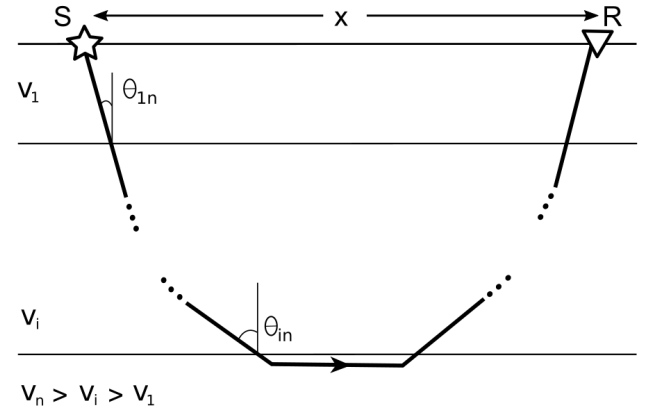
\includegraphics[width = 14cm, height = 8cm]{Imgs/RevisaoBibliografica/refracted_analytic.png}
	\caption{Esquema de modelagem analítica dos tempos da onda refratada. S e R são as posições da fonte e do receptor respectivamente. V e Z são as velocidades e as espessuras das camadas. $\theta$ é o angulo crítico das refrações e $i$ e $n$ se relacionam com a equação \ref{analytic_refractions}. Esquema geral com limitações entre posição de fonte e receptor, onde precisam estar na mesma profundidade, e velocidades, onde devem ser constantes lateralmente contendo camadas planas e horizontais.}
	\label{fig:refracted_analytic}
\end{figure}

\subsection*{Método clássico}

O método base utilizado para mensurar os avanços tanto em precisão quanto em eficiência computacional dos métodos numéricos que resolvem a equação eikonal foi a formulação de \citeonline{podvin1991finite}. Grandes contribuições foram publicadas em relação a localização não linear de epicentro e hipocentro de terremotos utilizando a formulação clássica, originadas com o trabalho de  \citeonline{wittlinger1993earthquake}, além das contribuições em tomografia e migração já mencionadas. A formulação de \citeonline{podvin1991finite} apresenta algumas limitações como instabilidade em camadas com alto ângulo de mergulho \cite{afnimar2000finite} e discrepância no cálculo dos tempos de trânsito utilizando a técnica da reciprocidade, onde a fonte assume a posição dos receptores e vice-versa \cite{tryggvason2006travel}. \citeonline{lomax2009earthquake} hospeda um repositório no \textit{GitHub}, de livre acesso, contendo os códigos originais para o cálculo da primeira chegada.  

A resolução da equação eikonal parte do princípio de Huygens, onde cada ponto pertencente a uma frente de onda pode se comportar como uma fonte que expande outra frente de onda. Então, a solução de \citeonline{podvin1991finite} aplica sistematicamente o princípio de Huygens considerando algumas possibilidades de propagação. Cada frente de onda, como por exemplo: difrações, refrações e onda direta, é calculada de forma independente sendo atualizada no volume de tempos como a opção de menor tempo entre as demais. Especificamente, operadores de diferenças finitas para casos 1D, 2D e 3D são aplicados, e considerando a indexação da Figura \ref{fig:voxel_full}, os principais operadores serão mostrados. 
\begin{figure}[H]
	\centering
	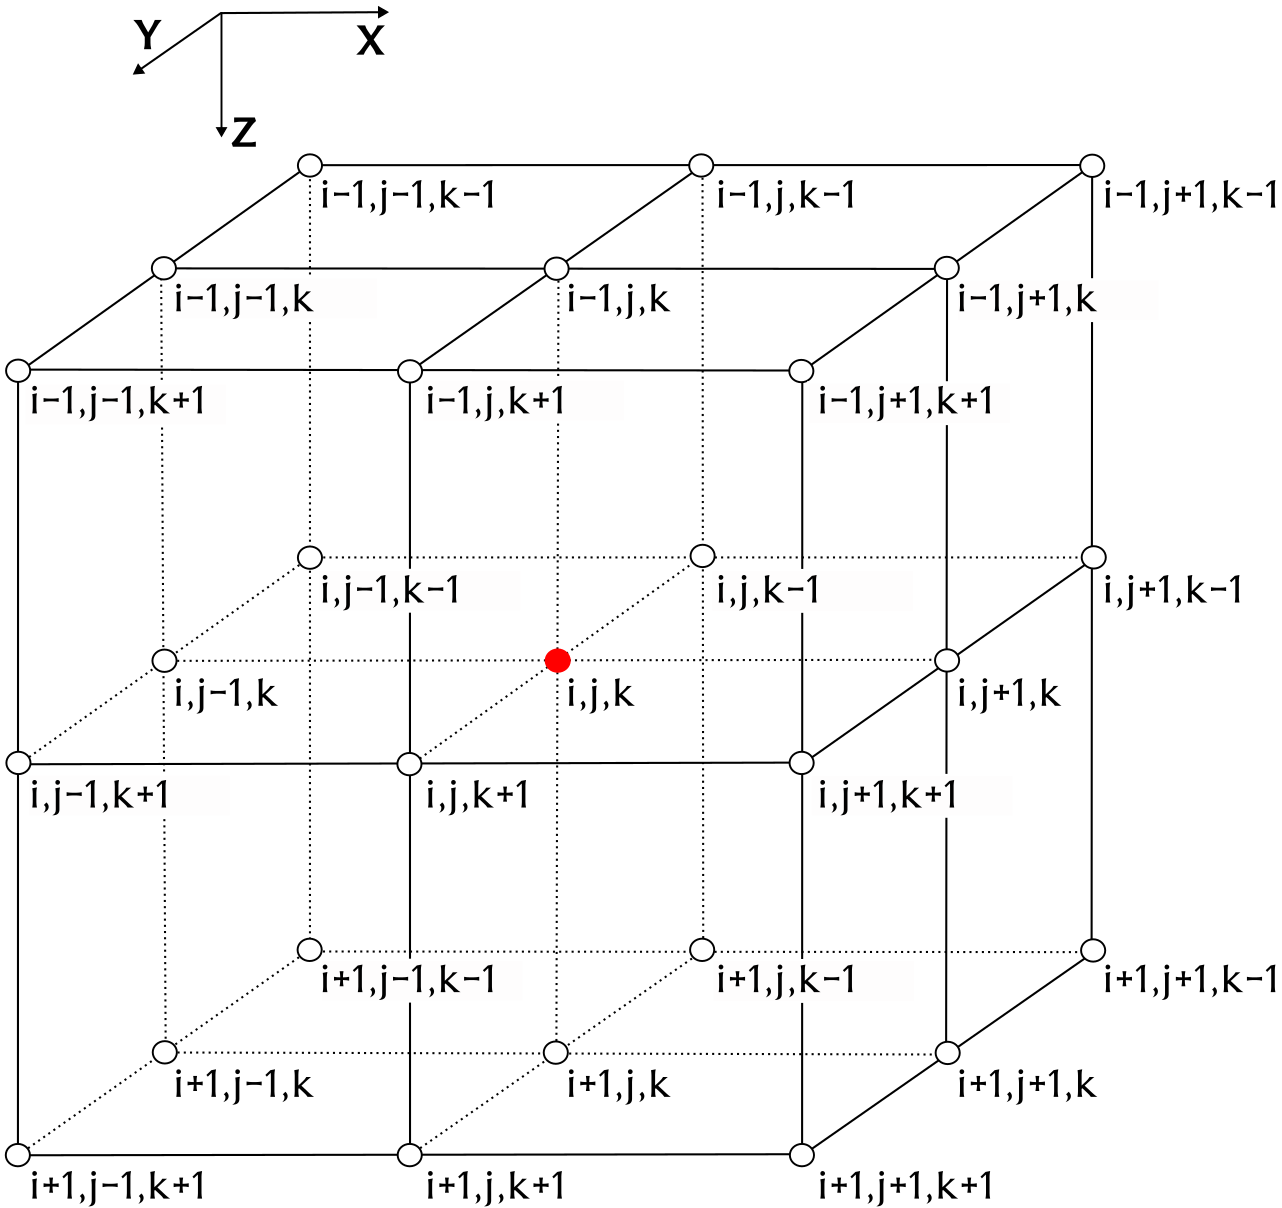
\includegraphics[width = 7cm, height = 6cm]{Imgs/RevisaoBibliografica/voxel_full.png}
	\caption{Esquema de indexação para o cálculo dos operadores de \citeonline{podvin1991finite}. O ponto vermelho é o alvo da propagação e os demais são seus vizinhos.}
	\label{fig:voxel_full}
\end{figure}
Os operadores 1D levam em consideração somente dois pontos, porém dependendo do ângulo de incidência as propriedades de vagarosidade devem ser escolhidas minuciosamente. O primeiro operador 1D se relaciona com a onda de corpo com propagação direta no sentido $(i,j-1,k) \to (i,j,k)$, seguindo os índices mostrados na Figura \ref{fig:voxel_full}, recebe a formulação
\begin{equation}
	T_{i,j,k} = T_{i,j-1,k} + dh\, \mathbf{min}(S_{i,j-1,k},\, S_{i,j-1,k-1},\, S_{i-1,j-1,k},\, S_{i-1,j-1,k-1}),
	\label{1d_head_wave}
\end{equation}   
\noindent onde $T$ e $S$ são os volumes de tempo e de vagarosidade respectivamente e $dh$ é o espaçamento espacial do modelo. Existem mais 5 direções para se aplicar o operador da equação \ref{1d_head_wave}, totalizando 6 operadores no total. Para o caso 1D em ondas difratadas, que ocorrem nas diagonais dos cubos, os operadores nos sentidos $(i-1,j-1,k-1) \to (i,j,k)$, $(i-1,j,k-1) \to (i,j,k)$ e $(i-1,j-1,k) \to (i,j,k)$, são respectivamente do seguinte formato
\begin{equation}
	\begin{cases}
		T_{i,j,k} = T_{i-1,j-1,k-1} + \sqrt{3}\,dh\,S_{i-1,j-1,k-1} \\
		T_{i,j,k} = T_{i-1,j,k-1} + \sqrt{2}\,dh\,\mathbf{min}(S_{i-1,j-1,k-1},\,S_{i-1,j,k-1}) \\
		T_{i,j,k} = T_{i-1,j-1,k} + \sqrt{2}\,dh\,\mathbf{min}(S_{i-1,j-1,k-1},\,S_{i-1,j-1,k}).
	\end{cases}
	\label{1D_diffractions}
\end{equation}
\noindent Como algumas frentes de onda se propagam entre dois cubos, a vagarosidade mínima é estrategicamente calculada para assegurar que a frente de onda se propagará pelo meio de maior velocidade, respeitando assim o princípio de Fermat. Operadores 1D de ondas difratadas são aplicados em 20 direções ao todo. Os operadores 2D seguem uma condição de iluminação sendo formulados, utilizando os pontos $(i-1,j,k-1)$ e $(i-1,j,k)$, a seguir
\begin{equation}
	\begin{cases}
		(1) \,\, S_{ref} = \mathbf{min}(S_{i-1,j-1,k-1},\, S_{i-1,j,k-1})  \\
		(2) \,\, 0 \le (T_{i-1,j,k} - T_{i-1,j,k-1}) \le \sqrt{2}\,dh\,S_{ref} \\
		(3) \,\, T_{i,j,k} = T_{i-1,j,k} + \sqrt{(dh\,S_{ref})^2 - (T_{i-1,j,k} - T_{i-1,j,k-1})^2},	
	\end{cases}
	\label{2D_operators}
\end{equation}
\noindent sendo $(1)$ a aplicação do princípio de Fermat, $(2)$ a condição de iluminação, $(3)$ o cálculo do tempo de trânsito e $S_{ref}$ é a vagarosidade de referência em cada operador. Para esse caso, vinte e quatro operadores são aplicados nas redondezas do ponto alvo $T_{i,j,k}$. Os operadores 3D são altamente condicionais, utilizam três pontos vizinhos e para cada cubo do modelo, três operadores são aplicados. Para melhor entendimento, a Figura \ref{fig:voxel3d} mostra as direções para um cubo, dos pontos utilizados para o cálculo dos operadores 3D seguindo a simbologia do trabalho de \citeonline{podvin1991finite}. 

\begin{figure}[H]
	\centering
	
	\subfloat[]{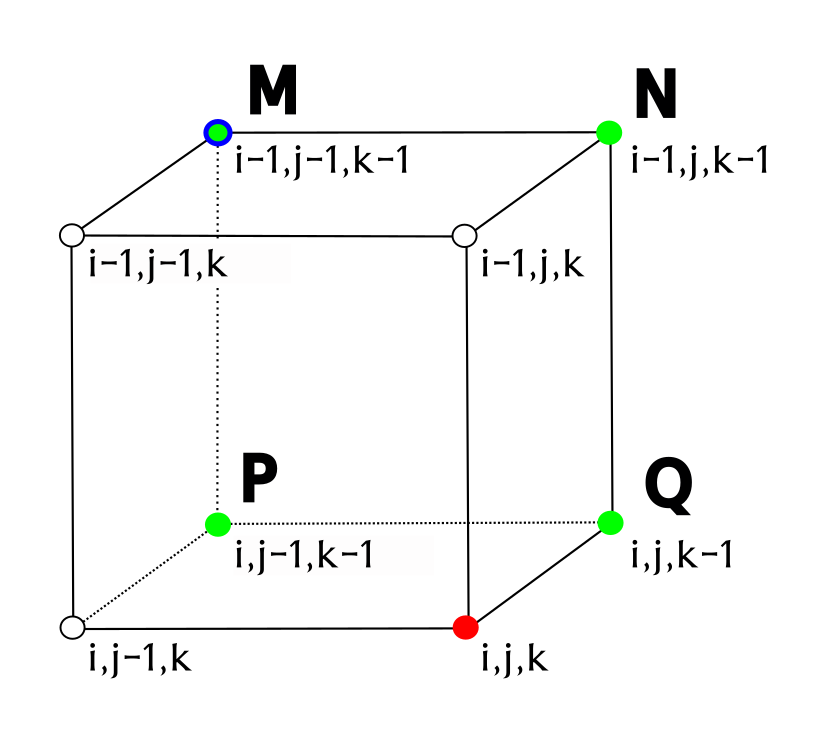
\includegraphics[width=4.5cm,height=4cm]{Imgs/RevisaoBibliografica/3D_xz.png}}
	\subfloat[]{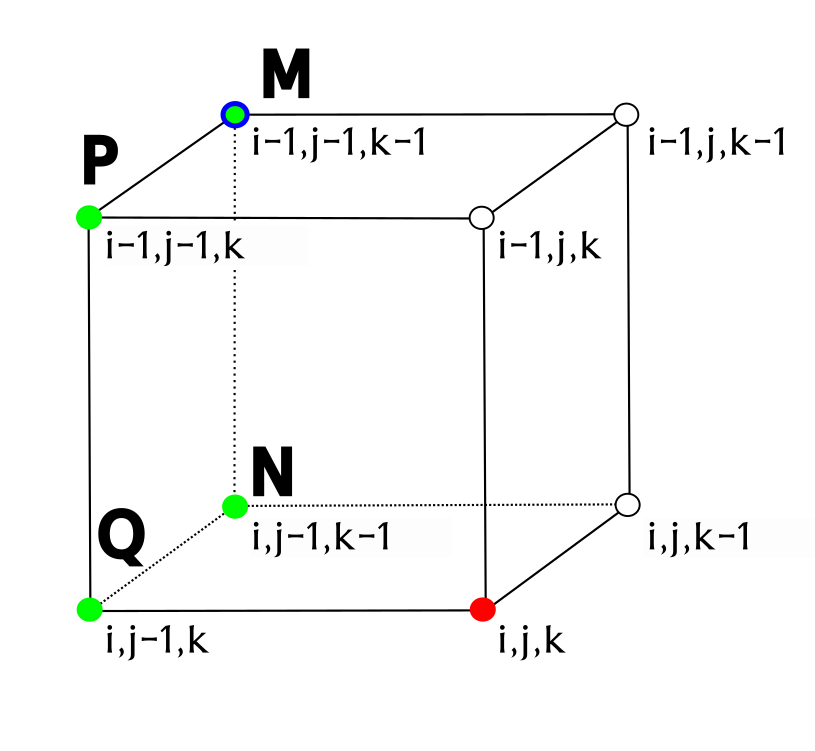
\includegraphics[width=4.5cm,height=4cm]{Imgs/RevisaoBibliografica/3D_yz.png}}
	\subfloat[]{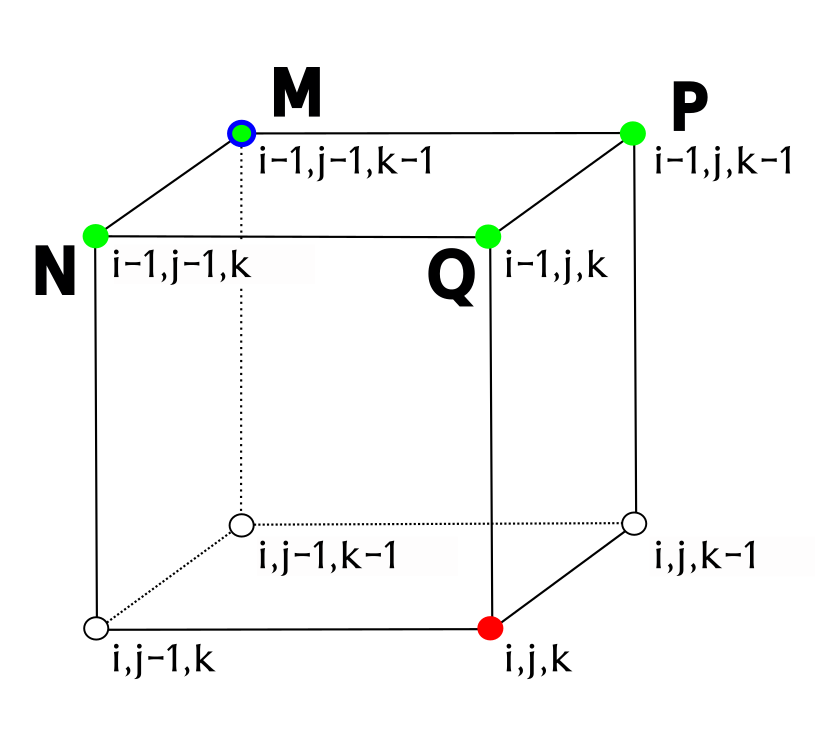
\includegraphics[width=4.5cm,height=4cm]{Imgs/RevisaoBibliografica/3D_xy.png}}
		
	\caption{Esquema de pontos utilizados na aplicação dos operadores 3D de \citeonline{podvin1991finite}. (a) plano xz, (b) plano yz e (c) plano xy. Pontos em verde são a vizinhança selecionada, o ponto em contorno azul é a posição da vagarosidade de referência, e o ponto em vermelho é o alvo da propagação.}
	\label{fig:voxel3d}
\end{figure}
\noindent Então, os operadores 3D seguem o mesmo padrão para quaisquer pontos (P,Q,M,N) selecionados corretamente. As formulações completas para uma composição de pontos mostrados na Figura \ref{fig:voxel3d}, podem ser escritas da maneira a seguir
\begin{multline}
	MNP \to T_{i,j,k}: \\ 
	M \le N \,\cap\, M \le P \\
	2(P-M)^2 + (N-M)^2 \le (dh\,S_{ref})^2 \\
	2(N-M)^2 + (P-M)^2 \le (dh\,S_{ref})^2 \\
	(N-M)^2 + (P-M)^2 + (N-M)(P-M) \ge 0.5(dh\,S_{ref})^2 \\
	T_{i,j,k} = N + P - M \sqrt{(dh\,S_{ref})^2 - (N-M)^2 - (P-M)^2}, \,\,\,\,\,\,\,\,\,\,\,\,\,\,\,\,\,\,\,\,\,
	\label{MNP-R}
\end{multline}
\begin{multline}
	QNP \to T_{i,j,k}: \\	
	N \le Q \,\cap\, P \le Q \\
	(Q-N)^2 + (Q-P)^2 + (Q-N)(Q-P) \le 0.5(dh\,S_{ref})^2 \\
	T_{i,j,k} = Q + \sqrt{(dh\,S_{ref})^2 - (Q-N)^2 - (Q-P)^2}, \,\,\,\,\,\,\,\,\,\,\,\,\,\,\,\,\,\,\,\,\,\,\,\,\,\,\,\,\,\,\,\,\,   
	\label{QNP-R}
\end{multline}
\begin{multline}
	NMQ \to T_{i,j,k}: \\	
	N \ge M \,\cap\, N-M \le Q-N \\
	2(Q-N)^2 + (N-M)^2 \le (dh\,S_{ref})^2 \\
	T_{i,j,k} = Q + \sqrt{(dh\,S_{ref})^2 - (Q-N)^2 - (N-M)^2}, \,\,\,\,\,\,\,\,\,\,\,\,\,\,\,\,\,\,\,\,\,\,\,\,\,\,\,\,\,\,\,\,
	\label{NMQ-R}
\end{multline}
\begin{multline}
	PMQ \to T_{i,j,k}: \\	
	P \ge M \,\cap\, P-M \le Q-P \\
	2(Q-P)^2 + (P-M)^2 \le (dh\,S_{ref})^2 \\
	T_{i,j,k} = Q + \sqrt{(dh\,S_{ref})^2 - (Q-P)^2 - (P-M)^2}. \,\,\,\,\,\,\,\,\,\,\,\,\,\,\,\,\,\,\,\,\,\,\,\,\,\,\,\,\,\,\,\,
	\label{PMQ-R}
\end{multline}

A resolução da equação eikonal é iterativa e a cada iteração é necessário que uma frente de onda se expanda passando pelos pontos onde o tempo de trânsito é desconhecido. Inicialmente, o volume dos tempos de trânsito recebe o valor zero na fonte e um valor tendendo ao infinito nas demais posições. Os pontos vizinhos à posição da fonte são inicializados utilizando a equação da cinemática clássica $t = x / v$, considerando que cada bloco do modelo possui um valor de velocidade constante. Para posições de fonte irregulares, ou seja, posições que não pertencem a nenhum ponto da malha, o tempo da fonte é inicializado de acordo com a distância entre a fonte e o ponto da malha mais próximo. Assim, a solução iterativa de \citeonline{podvin1991finite} pode propagar o tempo inicial para as demais posições automaticamente. Após a inicialização, um volume lógico é inicializado com valores de verdadeiro e falso, sendo verdadeiro as posições que convergiram para um tempo de trânsito aceitável e falso, para posições que ainda não convergiram. O número de iterações depende da distância, em pontos de malha, entre a posição da fonte e as extremidades do modelo de velocidade, sendo a maior distância em pontos de malha que houver. Durante as iterações, todos os pontos do modelo são acessados, porém as equações são calculadas somente onde o volume lógico indica necessidade de atualização. A partir do momento que o tempo de trânsito de um certo ponto atinge a confiabilidade dada por uma tolerância, novos pontos são acionados como verdadeiros e assim, os operadores computam novos tempos em regiões ainda não exploradas até completar toda a extensão do modelo de velocidades. Para registrar os tempos de trânsito em cada posição de receptor, basta coletar o tempo do volume de tempos de trânsito e para posições irregulares, a interpolação tri-linear foi utilizada para resolver o problema.  

A solução de \citeonline{podvin1991finite} é altamente paralelizável. Um processo que pode ser paralelizado é aquele que possui problemas pequenos que podem ser resolvidos de forma independente e assim simultaneamente. O algoritmo desenvolvido pelo autor deste trabalho, para resolver a equação eikonal utilizando os operadores de \citeonline{podvin1991finite}, pode ser encontrado na plataforma de compartilhamento de código aberto GitHub.  

\subsection*{\textit{Fast Iterative Method}}

Original de \citeonline{jeong2008fast}, o \textit{Fast Iterative Method} (FIM) é uma metodologia que utiliza uma frente de onda variável que se adapta ao modelo de velocidades, tornando assim uma frente de onda mais realística. FIM é uma técnica de resolução baseada nas formulações de frente de onda expansivas como o \textit{Fast Marching Method} (FMM). O FMM, formulado por \citeonline{sethian1999fast}, possui grandes aplicabilidades em geociências como os trabalhos de \citeonline{sethian19993, rawlinson2004multiple, lelievre2011computing, jiang2021fast} e até a presente data deste trabalho ainda é explorado com diferentes implementações \cite{white2020pykonal, chenpyekfmm2023}. Por outro lado o FIM, ainda pouco estudado na área de geociências, possui vantagens computacionais em relação ao FMM, onde em cada iteração se resolve uma ordenação com a estrutura de dados \textit{heap} para atualizar a frente de onda irregular (\textit{heap sort}). O FIM não depende de estruturas de dados e cada ponto pertencente à frente de onda irregular é resolvido simultaneamente. A estratégia do FMM pode ser eficiente em computação sequencial, porém torna-se ineficiente utilizando paralelismo de larga escala até o momento da publicação de \citeonline{jeong2008fast}. Alguns anos depois, \citeonline{yang2017highly} resolvem a aplicabilidade do FMM, porém essa solução não foi considerada neste estudo. A ênfase neste trabalho foi a experimentação da formulação de \citeonline{jeong2008fast}, ainda pouco explorada. 

Outras contribuições como a implementação do FIM em diferentes discretização o modelo como malhas triangulares e tetraédricas \cite{fu2011fast, fu2013fast} e melhoria da eficiência computacional \cite{dang2014fast, hong2016multi, hong2022mg} foram desenvolvidas. A discussão em relação à imprecisão dos tempos de trânsito utilizando a formulação de \citeonline{jeong2008fast} foi destacada por \citeonline{cai2023improved}. A modificação considerada foi aumentar a quantidade de pontos vizinhos para o cálculo dos tempos de trânsito sem diminuição significativa da eficiência computacional, porém a melhoria proposta não foi acoplada a este trabalho. 

A ideia principal do FIM é resolver a equação de Eikonal utilizando uma lista de ativos que contempla os pontos da frente de onda, sem manter estruturas de dados caras, como um \textit{heap} por exemplo. O método de \cite{jeong2008fast} mantém um
relacionamento mais flexível e atualiza todos os pontos da malha contidos na lista ativa simultaneamente usando computação paralela. Durante cada iteração, expandimos a lista de pontos ativos e a frente de onda expande para incluir todos os pontos que podem ser afetados pelas atualizações atuais.  Um ponto contido na frente de onda pode ser removido da lista ativa quando sua solução estiver atualizada em relação para seus vizinhos (ou seja, convergiu). Somente os pontos contidos na lista de ativos são acessados em cada iteração e esses pontos podem ser atualizados simultaneamente. A inicialização se assemelha com o método de resolução da equação eikonal apresentado na seção anterior \cite{podvin1991finite}, onde a posição da fonte recebe o valor zero e os demais pontos no volume de tempo de trânsito recebe um valor alto.

A versão utilizada neste trabalho decompõe o modelo em pequenos blocos contendo 4x4x4 amostras de malha, versão esta chamada de \textit{block}-FIM. Cada bloco se comporta como um ponto de malha na frente de onda expansiva, e assim a lista se preenche com blocos ativos ao invés de pontos. Nessa estratégia, se utiliza otimizações específicas de computação paralela comentadas no trabalho de \citeonline{jeong2008fast}, onde o algoritmo original \textit{block}-FIM pode ser encontrado no Github, num repositório hospedado pelos próprios autores.

\begin{algorithm}[H]
	\caption{Equação principal do \textit{Fast Iterative Method}}
	\footnotesize
	\SetAlgoLined
	\Entrada{$T$, $\,S_{i,j,k}$, $\,dh$} 
	\Saida{$T_{i,j,k}$}
	\Inicio
	{	
		$a = \mathbf{min}(T_{i-1,j,k}, T_{i+1,j,k})$ \\
		$b = \mathbf{min}(T_{i,j-1,k}, T_{i,j+1,k})$ \\
		$c = \mathbf{min}(T_{i,j,k-1}, T_{i,j,k+1})$ \\
		
		$a,b,c \leftarrow \mathbf{ordene}(a,b,c)\,\, \text{tal que}\,\, a > b > c$ \\
		\Se{$c < \infty$}
		{
			$T_{i,j,k} \leftarrow c + dh\,S_{i,j,k} \\
			
			\Se{$T_{i,j,k} > b$}
			{
				$T_{aux} = 0.5(b + c + \sqrt{2(dh\,S_{i,j,k})^2 - (b - c)^2})$ \\
				
				\Se{$T_{aux} > b$}
				{
					$T_{i,j,k} = T_{aux}$ \\	
				}
				 
				\Se{$T_{i,j,k} > a$}
				{
					$T_{aux} = \left((a + b + c) + \sqrt{2(a(b-a) + b(c-b) + c(a-c))}\right) / 3$ \\	
					
					\Se{$T_{aux} > a$}
					{
						$T_{i,j,k} = T_{aux}$ \\ 
					}
				}	
			}
		}
	}
\end{algorithm}

O algoritmo 1 mostra o núcleo de resolução do FIM, onde o primeiro passo é ordenar as diferenças dos tempos de trânsito dos vizinhos diretos do ponto alvo $T_{ijk}$ e aplicar condições de iluminação desenvolvidas empiricamente por \citeonline{jeong2008fast}. Para registrar os tempos das primeiras chegadas, as posições dos receptores são projetadas no volume de tempo de trânsito e para posições irregulares, fora da malha, a interpolação tri linear é utilizada, assim como mencionado na seção anterior.  

\subsection*{\textit{Fast Sweeping Method}}

Original de \citeonline{zhao2005fast}, o \textit{Fast Sweeping Method} (FSM) é uma formulação que utiliza os operadores clássicos aplicados desde o trabalho de \citeonline{vidale1988finite}, porém aplica uma ordem específica de atualização. Essa forma pode ser chamada de iterações de Gauss-Seidel, onde o domínio computacional é acessado utilizando diferentes direções. Para o caso 3D, oito direcionamentos são aplicados resolvendo as equações conhecidas e desenvolvidas por \citeonline{vidale1988finite, afnimar2000finite}. As direções específicas a serem percorridas são descritas a seguir
\begin{center}
\noindent (1) i = 1:Nx;$\,\,\,\,$ j = 1:Ny;$\,\,\,\,$ k = 1:Nz,$\,\,\,\,\,\,\,\,$ (2) i = Nx:1;$\,\,\,\,$ j = 1:Ny;$\,\,\,\,$ k = 1:Nz, \newline 
\noindent (3) i = 1 Nx;$\,\,\,\,$ j = Ny:1;$\,\,\,\,$ k = 1:Nz,$\,\,\,\,\,\,\,\,$ (4) i = 1:Nx;$\,\,\,\,$ j = 1:Ny;$\,\,\,\,$ k = Nz:1, \newline
\noindent (5) i = 1:Nx;$\,\,\,\,$ j = Ny:1;$\,\,\,\,$ k = Nz:1,$\,\,\,\,\,\,\,\,$ (6) i = Nx:1;$\,\,\,\,$ j = 1:Ny;$\,\,\,\,$ k = Nz:1, \newline 
\noindent (7) i = Nx:1;$\,\,\,\,$ j = Ny:1;$\,\,\,\,$ k = 1:Nz,$\,\,\,\,\,\,\,\,$ (8) i = Nx:1;$\,\,\,\,$ j = Ny:1;$\,\,\,\,$ k = Nz:1. $\,\,\,\,\,\,\,\,\,\,\,\,\,$
\end{center}
\noindent onde a numeração é a ordem de aplicação para um modelo limitado por (Nx, Ny, Nz) amostras. Com essa ordenação, os operadores de diferenças finitas podem ser derivados somente para uma única direção, variando com indicadores direcionais para a vagarosidade e para os tempos de trânsito vizinhos. A contribuição utilizada neste trabalho se origina de \citeonline{noble2014accurate}, onde novos operadores são aplicados para aprimorar a precisão dos tempos de trânsito. A inovação foi considerar a forma expandida dos operadores de oito pontos de \citeonline{vidale1988finite}, onde a seguinte derivada do tempo $T$ em relação a direção $x$ é considerada    
\begin{equation}
	\dfrac{\partial T}{\partial x} \approx \left(\dfrac{T_{i,j,k} - T_i}{4\, dh_x}\right),
	\label{fsm_8p_derivative}
\end{equation}
\noindent onde $T_i$ são os sete pontos na redondeza de $T_{i,j,k}$ para o primeiro quadrante, ou seja,
\begin{equation}
	T_i = - T_{i-1,j,k} + T_{i,j-1,k} - T_{i-1,j-1,k} + T_{i,j,k-1} - T_{i-1,j,k-1} + T_{i,j-1,k-1} - T_{i-1,j-1,k-1}.
\end{equation} 
\noindent Aplicando a equação \ref{fsm_8p_derivative} para as outras direções e substituindo na equação \ref{eikonal_full}, obtém-se
\begin{equation}
	\left(\dfrac{T_{i,j,k} - T_i}{4\,dh_x}\right)^2 + \left(\dfrac{T_{i,j,k} - T_j}{4\,dh_y}\right)^2 + \left(\dfrac{T_{i,j,k} - T_k}{4\,dh_z}\right)^2 = S^2_{i,j,k}
	\label{quadratic}
\end{equation}
\noindent onde $dh_x$,$dh_y$ e $dh_z$ são os parâmetros de discretização espaciais para as direções cartesianas. Embora a formulação de \citeonline{noble2014accurate} disponibiliza a opção de heterogeneizar os espaçamentos da malha, porém o espaçamento fixo foi utilizado neste trabalho. A partir da equação de segundo grau \ref{quadratic}, onde $T_{i,j,k}$ é a incógnita, duas soluções são possíveis, entretanto somente a de maior é considerada. \citeonline{noble2014accurate} mostram os coeficientes que resolvem o problema \ref{quadratic}, apresenta os operadores em sua forma cartesiana e esférica. O autor da formulação hospeda um repositório no GitHub com os códigos desenvolvidos para gerar os resultados publicados. Apesar da utilização de operadores em coordenadas esféricas próximos da fonte para melhorar a precisão dos tempo de trânsito, somente os operadores cartesianos foram aplicados no desenvolvimento deste trabalho.        

A primeira forma de paralelização do FSM foi desenvolvida por \citeonline{zhao2007parallel}, porém limitações para grande quantidade de processos simultâneos foram encontradas, fazendo com que o tempo de execução se estabelecesse constante com o aumento do poder computacional. \citeonline{detrixhe2013parallel} desenvolvem uma técnica que supera o problema encontrado na formulação de \citeonline{zhao2007parallel}, onde a performance é proporcional ao aumento computacional. Basicamente, a direção de percorrimento no modelo de tempo de trânsito acontece em planos diagonais e cada ponto desses planos podem ser atualizados simultaneamente. O modelo de propriedades de formato cúbico ou paralelepipédico possui oito quinas, então a partir de cada quina, a direção de percorrimento segue de uma quina origem até quina espelhada oposta, percorrendo cada plano diagonal e aplicando os operadores de diferenças finitas. Por consequência da implementação dos operadores 3D de precisão, somente três formas de resolução são aplicadas no núcleo do FSM. O primeiro segue o formado dos operadores 1D de \citeonline{podvin1991finite}, baseados na cinemática clássica (equação \ref{1d_head_wave}), o segundo segue os operadores 2D de quatro pontos apresentados por \citeonline{vidale1988finite} e o terceiro é a expansão do operador 3D, também apresentado por \citeonline{vidale1988finite}. Com a diminuição dos operadores no núcleo da modelagem, o caso sequencial é viável, porém neste trabalho a forma paralelizada de \citeonline{detrixhe2013parallel} foi aplicada.  

\section{Inversão tomográfica}

Nas seções anteriores a modelagem direta foi explorada exemplificando maneiras de como calcular o dado de primeira chegada, ou seja as ondas transmitidas e refratadas. Contudo, na natureza a subsuperfície não é conhecida e para realizar os estudos de investigação, somente os registros sísmicos na superfície terrestre são obtidos. A tomografia sísmica pode ser explorada utilizando diferentes formas de onda, como por exemplo as ondas refletidas, difratadas e refratadas. \citeonline{murphy1999manual} resumem as estratégias da tomografia de reflexão, \citeonline{santos2012tomography} comentam sobre as vantagens da tomografia de difração, \citeonline{almeida2013tomografia} e \citeonline{capucci2013tomografia} desenvolvem experimentos relacionados com a tomografia de refração. Todos esses casos partem do mesmo objetivo: minimizar a diferença entre o dado observado e o dado calculado.  Aspectos práticos do método tomográfico são amplamente descritos no trabalho de \citeonline{sain2023active}. De maneira geral o dado artificial pode ser gerado pela equação
\begin{equation}
	d^{cal} = \displaystyle\int_{raio} s\,dr = g(m),
\end{equation}
\noindent onde $d^{cal}$ é o dado calculado que pode ser estimado a partir da soma infinitesimal de fragmentos do raio $dr$ vezes a vagarosidade $s$. O operador de modelagem direta $g(m)$ tem características não lineares pois os raios propagados dependem do modelo de vagarosidade $m$ \cite{seo2012nonlinear}. Este modelo pode representar diferentes formatos no momento da inversão, desde células ou pontos de malha até equações analíticas como no trabalho de \citeonline{daiana} que parametrizam o modelo com a soma de funções de base radial, sendo que para este trabalho a discretização por pontos de malha foi considerada. 

A função objetivo da tomografia utilizando a norma euclidiana de ordem 2 pode ser formulada da seguinte maneira
\begin{equation}
	\chi(m) = \dfrac{1}{2}\left[d^{obs} - g(m)\right]^T\left[d^{obs} - g(m)\right] = \displaystyle\sum_{n = 0}^N(d^{obs}_n - g_n(m))^2, 
	\label{objectiveFunction}
\end{equation} 
\noindent sendo $d^{obs}_n$ o dado observado para cada estação $n$. De forma clássica, a inversão tomográfica pode ser linearizada por um modelo inicial e após a aplicação da expansão em série de Taylor de segunda ordem da equação \ref{objectiveFunction}, pode-se se resolver iterativamente sistemas lineares utilizando a aproximação de Gauss-Newton \cite{tarantola2005inverse, menke2018geophysical, aster2018parameter}. O sistema linear é formado pela aproximação da matriz Hessiana, a segunda derivada, e pelo gradiente da equação \ref{objectiveFunction}. O objetivo é estimar as pequenas variações do modelo de vagarosidade de acordo com a diferença entre o dado observado e calculado de forma iterativa. Em formato de equação, o núcleo da inversão pode ser formulado pela seguinte expressão 
\begin{equation}
	G^TG \Delta m_p = G^T\Delta d_p, 		
	\label{linearSystem}
\end{equation} 
\noindent onde $G^TG$ é a aproximação da Hessiana, $\Delta m_p$ é a variação do modelo na iteração $p$, $\Delta d_p$ é a variação do dado na iteração $p$ e $G^T\Delta d$ é a aproximação do gradiente da equação \ref{objectiveFunction}. A matriz $G$ é esparsa contendo as distâncias percorridas para cada raio por elemento de modelo a cada iteração. Como os elementos de modelo são cubos ou paralelepípedos no caso 3D, a matriz $G$ tem o tamanho em linhas: a quantidade de raios projetados na simulação, e em colunas: a quantidade de elementos de modelo. Resolvendo o problema iterativamente, no instante inicial um modelo a priori é considerado e a modelagem por equação eikonal é realizada. Com o volume de tempo de trânsito, o traçado de raios pode ser realizado a partir de que os raios se propaguem perpendicularmente às isócronas de tempo \cite{vidale1988finite}. O traçado de raios via equação eikonal pode ser formulado, em três dimensões, da maneira a seguir
\begin{equation}
	\begin{cases}
		x_i = x_{i-1} + \alpha\,\, \partial_x\, T \,/\, ||\nabla T|| \\ 
		y_i = y_{i-1} + \alpha\,\, \partial_y\, T \,/\, ||\nabla T|| \\ 
		z_i = z_{i-1} + \alpha\,\, \partial_z\, T \,/\, ||\nabla T||. 
	\end{cases}
	\label{rayTracing}
\end{equation}
\noindent Considerando um raio possuindo coordenadas $x$,$y$ e $z$ na posição $i$, a próxima coordenada pode ser estimada a partir da posição anterior somado a um tamanho de passo $\alpha$ definido em metros multiplicado pela derivada do tempo de trânsito normalizada.  

Para garantir uma solução única em uma equação normal, onde a função objetivo pode ser formulada por
\begin{equation}
	\chi(m) = \text{min}||d^{obs} -g(m)||^2_2,
\end{equation}
\noindent é necessário que a matriz Hessiana tenha posto completo, ou seja, que suas colunas (ou linhas) sejam linearmente independentes. No entanto, em problemas geofísicos, é comum que a matriz do sistema tenha um determinante próximo de zero, o que indica falta de posto completo. Isso torna o problema inverso geofísico mal posto, apresentando instabilidade e falta de unicidade na solução. A instabilidade refere-se à alta variabilidade do modelo estimado quando há pequenas variações nos dados observados. A falta de unicidade implica que existem vários conjuntos modelos estimados que produzem os mesmos dados observados. Na prática, isso significa que há vários modelos diferentes que minimizam a função de objetivo. Problemas inversos na geofísica geralmente são mal postos devido ao ruído nos dados observados e à própria natureza do problema inverso. Para lidar com esses problemas, é essencial usar regularização, um procedimento matemático que contorna a instabilidade e a falta de unicidade em problemas inversos mal postos. A regularização impõe restrições aos parâmetros estimados, buscando encontrar um conjunto de parâmetros que se ajustem aos dados observados e satisfaçam as restrições estabelecidas, que podem ser de natureza geológica ou matemática e são introduzidas por meio de funções regularizadoras. Mais informações sobre regularização de maneira geral, os trabalhos de \citeonline{tarantola2005inverse} e \citeonline{aster2018parameter} são excelentes para consulta.   

A regularização de Tikhonov foi utilizada neste trabalho e o equacionamento geral do esquema pode ser formulado da seguinte maneira
\begin{equation}
	\chi(m) = \text{min}||d^{obs} - g(m)||^2_2 +\lambda||Rm||^2_2,
\end{equation}
\noindent onde $\lambda$ é um escalar que controla a importância relativa da regularização e $R$ representa uma matriz com operadores de derivada. O problema \ref{linearSystem} regularizado pode ser equacionado no formato a seguir
\begin{equation}
	(G^TG + \lambda^2 R^TR)\Delta m = G^T \Delta d.
\end{equation}
\noindent A regularização de Tikhonov pode ser aplicada em ordens específicas de acordo com o operador de derivada. A matriz $R$ de ordem zero pode escrita da seguinte forma
\begin{equation}
	R_0 = 
	\begin{bmatrix}
		1 & 0 & 0 & \cdots & 0 \\
		0 & 1 & 0 & \cdots & 0 \\
		0 & 0 & 1 & \cdots & 0 \\
		\vdots & \vdots & \vdots & \ddots & \vdots \\
		0 & 0 & 0 & \cdots & 1 \\
	\end{bmatrix}
	_{M\times M},
\end{equation}
\noindent onde seu tamanho depende da quantidade dos parâmetros do modelo $M$. Altas ordens de derivada podem ser aplicadas na regularização de Tikhonov, porém as mais comuns são de zero, primeira e segunda ordens. Neste trabalho a aplicação da regularização de Tikhonov de segunda ordem foi aplicada pois em \citeonline{bulhoes2021efeitos}, esse tipo de regularização demonstrou uma convergência mais rápida em relação às ordens inferiores. Para efeito ilustrativo, a matriz $R$ com operadores de segunda ordem pode ser formulada da seguinte maneira
\begin{equation}
	R_2 = 
	\begin{bmatrix}
		1      & -2     & 1      & 0      & 0      & \cdots & 0      & 0      & 0 \\
		0      & 1      & -2     & 1      & 0      & \cdots & 0      & 0      & 0 \\
		0      & 0      & 1      & -2     & 1      & \cdots & 0      & 0      & 0 \\
		\vdots & \vdots & \vdots & \vdots & \vdots & \ddots & \vdots & \vdots & \vdots \\
		0      & 0      & 0      & 0      & 0      & \cdots & 1      & -2     & 1 \\
	\end{bmatrix}
	_{(M-2)\times M},
\end{equation}
\noindent com tamanho de linhas reduzidas de acordo com a ordem do operador. Mais exemplos clássicos de regularização aplicados no método da tomografia sísmica podem ser encontrados no trabalho de \citeonline{yao1999practical}. Uma contribuição interessante de regularização é a aplicação conjunta de dois regularizadores: Tikhonov e variação total. \citeonline{lin2014acoustic} iniciam os estudos para inversão completa do campo de onda, \citeonline{jiang20183d} aplicam a regularização de Tikhonov para estabilizar o problema inverso e em conjunto, aplicam a regularização por variação total para recuperar os altos contrastes, por consequência da regularização de Tikhonov possuir efeitos suavizadores.   

Em problemas tomográficos não lineares a cada iteração se resolve um sistema linear, que dependendo dos aspectos do dado observado e da discretização do modelo a aproximação da matriz Hessiana pode se tornar inviável computacionalmente. Para resolver o problema de forma barata, suas estratégias podem ser aplicadas: a técnica de resolver um problema de mínimos quadrados sem calcular a matriz Hessiana e o armazenamento de matrizes esparsas. A matriz $G$ contendo as distâncias percorridas pelos raios a cada célula pertencente ao modelo de velocidade têm aspectos esparsos, pois cada raio ilumina poucas células no modelo de velocidade. Então a matriz $G$ pode ser ordenada utilizando alguma técnica de armazenamento esparso. A técnica utilizada neste trabalho foi armazenas as coordenadas completas em duas listas e a terceira lista contendo os elementos não nulos da matriz. Essa técnica é relativamente mais cara do que as demais existentes, como a CSR - \textit{compress sparse row} ou a CSC - \textit{compress sparse column}, porém as operações de multiplicação são mais amigáveis de se implementar. Apesar da matriz $G$ possuir características esparsas, a esparsidade da matriz Hessiana não é alta. A técnica de resolução do problema de mínimos quadrados sem o cálculo da matriz $G^TG$ se torna extremamente aplicável no caso da tomografia 3D \cite{hestenes1952methods, saad2003iterative}. O equacionamento da resolução do problema de mínimos quadrados pode ser encontrada no trabalho de \citeonline{capucci2013tomografia}. 

A estrutura do algoritmo de tomografia pode ser ilustrada na figura \ref{tomography_chart}. Inicialmente a leitura dos dados observados é realizada. Após a importação do modelo inicial, a solução eikonal é efetuada para coletar os tempos de trânsito em cada receptor, gerando o dado calculado. Assim o resíduo pode ser efetuado e em seguida a otimização pode ser realizada com a solução do problema de mínimos quadrados, recuperando a variação do modelo de vagarosidade. Uma etapa adicional pode ser aplicada para suavizar o modelo de vagarosidade caso a recuperação tenha gerado artefatos ou se a malha de inversão for esparsa. A suavização utilizando a equação gaussiana foi utilizada neste trabalho. Em seguida, a atualização do modelo pode ser efetuada adicionando a variação recuperada ao modelo de vagarosidade da iteração anterior. 

A etapa de convergência pode considerar o número de iterações desejadas ou uma tolerância específica da norma da função objetivo como critério de parada. Se a convergência for significativa respeitando uma das condições, o processo exporta o modelo final de velocidade e a curva de convergência, e se não respeitar as condições, o processo tomográfico realiza uma nova iteração utilizando o modelo atualizado.      

\begin{figure}[H]
	\centering
	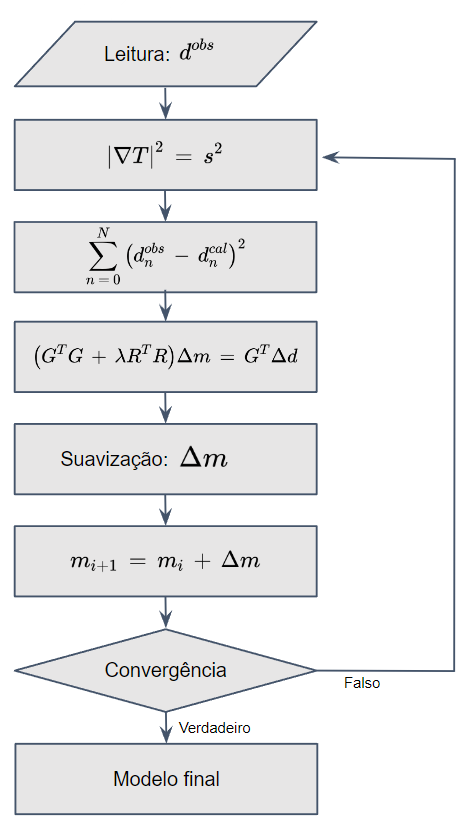
\includegraphics[width=7.5cm, height=12cm]{Imgs/RevisaoBibliografica/tomography_chart.png}
	\caption{Esquema tomográfico de acordo com o equacionamento apresentado.}
	\label{tomography_chart}
\end{figure}

\subsection*{Obtenção do dado observado}

O sismograma completo adquirido no campo são é completamente necessário para a realização da tomografia, somente os pares ($x$,$t$) que compõem as primeiras chegadas. A recuperação dessas posições podem ser recuperadas manualmente, com a seleção manual da primeira chegada. Contudo, essa estratégia consome tempo demasiado em aquisições de larga escala. Duas estratégias são capazes de substituir a abordagem manual de seleção da primeira chegada: as formulações baseadas em amplitude, energia e espectro dos dados e as formulações por aprendizado de máquina e inteligência artificial. \citeonline{sabbione2010automatic} sumarizam as principais estratégias analíticas para a seleção de dados de primeira chegada e mais atualmente, \citeonline{ayub2021comparative} comparam as técnicas de aprendizado de máquina e inteligência artificial desenvolvidas. \citeonline{yuan2022segnet} apresentam uma abordagem interessante para solucionar os problemas de traços irregulares e altos ruídos em seleções automáticas de primeira chegada utilizando inteligencia artificial, já que a abordagem analítica pode gerar artefatos com dados ruidosos. 

Considerando a utilização de dados sintéticos, a formulação aplicada neste trabalho é analítica baseada no somatório da energia do dado em janelas de percorrimento temporal. \citeonline{pan2019automatic} calcula dois parâmetros relacionados com o traço sísmico 
\begin{equation}
	A = \displaystyle\sum_{k=i-n}^{k=i} T_k;\,\,\,\,\,\, B = \displaystyle\sum_{k=i}^{k=i+n} T_k, 
\end{equation} 
\noindent onde $i$ é a amostra de tempo atual, $n$ é o tamanho da janela temporal em amostras e $T_k$ é a amplitude do traço na amostra $k$. Assim as variáveis $A$ e $B$ são aplicadas na seguinte equação
\begin{equation}
	S = |(B / A)\times(B - A)|,
\end{equation} 
\noindent sendo $S$ a indicação de existência de primeiras chegadas no dado. \citeonline{qin2021first} adiciona novos termos para se obter indicações de primeiras chegadas mais precisas formulando a equação
\begin{equation}
	S = S\times(B + A)\times(B/A)\times(B-A)/(n+i)^2, 
	\label{automatic_picking}
\end{equation}
\noindent onde $n$ e $i$ são o tamanho da janela em amostras e é a amostra de tempo atual. Com a equação \ref{automatic_picking}, aplicando traço a traço e a cada passo no tempo se observa um sismograma com as mudanças de energia em forma de funções denta de Dirac, sendo que a primeira ocorrência será o tempo da primeira chegada.   